\documentclass[a4paper,12pt]{article}
\usepackage{amsmath}
\usepackage{graphicx}
\begin{document}
\title{Homework 4}
\author{Matt Forbes}
\date{October 26, 2010}
\maketitle
\section*{3.20}
\subsection*{\(a)\) Using subproblem}
Original problem:
\begin{center}
\begin{tabular}{| c | c  c  c |}
\hline
0 & 4 & 0 & -1\\
\hline
-1 & 1 & 1 & -1\\
1 & -1 & 1 & 0\\
\hline
\end{tabular}
\end{center}

Phase 0:
\begin{center}
\begin{tabular}{| c | c  c  c |}
\hline
4 & 0 & 0 & -1\\
\hline
-1 & 1 & 0 & -0.5\\
0 & 0 & 1 & -0.5\\
\hline
\end{tabular}
\end{center}

Now form subproblem with obj. function as row 1, and pivot:
\begin{center}
\begin{tabular}{| c | c  c  c |}
\hline
6 & -2 & 0 & 0\\
\hline
2 & -2 & 0 & 1\\
1 & -1 & 1 & 0\\
\hline
\end{tabular}
\end{center}

\subsection*{\(b)\) Using artificial problem}
Initial artificial problem:
\begin{center}
\begin{tabular}{| c | c  c  c  c  c |}
\hline
0 & 0 & 0 & 0 & 1 & 1\\
\hline
-1 & 1 & 1 & -1 & 1 & 0\\
1 & -1 & 1 & 0 & 0 & 1\\
\hline
\end{tabular}
\end{center}

Pivoted to optimal form (feasible because d = 0):
\begin{center}
\begin{tabular}{| c | c  c  c  c  c |}
\hline
0 & 0 & 0 & 0 & 1 & 1\\
\hline
2 & -2 & 0 & 1 & -1 & 1\\
1 & -1 & 1 & 0 & 0 & 1\\
\hline
\end{tabular}
\end{center}

Revert to original problem's objective function:
\begin{center}
\begin{tabular}{| c | c  c  c |}
\hline
0 & 4 & 0 & -1\\
\hline
2 & -2 & 0 & 1\\
1 & -1 & 1 & 0\\
\hline
\end{tabular}
\end{center}

\section*{3.24}
Make one pivot on the original matrix such that it decreases the objective function by the smallest amount.\\\\
Original Tableau:
\begin{center}
\begin{tabular}{| c | c  c  c  c  c  c |}
\hline
-9 & 0 & 4 & 5 & 0 & 2 & 0\\
\hline
4 & 1 & 2 & 4 & 0 & 1 & 0\\
5 & 0 & 3 & 1 & 1 & -1 & 0\\
\hline
\end{tabular}
\end{center}

After the pivot:
\begin{center}
\begin{tabular}{| c | c  c  c  c  c  c |}
\hline
-14 & -1.25 & 1.5 & 0 & 0 & 0.75 & 0\\
\hline
1 & 0.25 & 0.5 & 1 & 0 & 0.25 & 0\\
4 & -0.25 & 2.5 & 0 & 1 & -1.25 & 0\\
\hline
\end{tabular}
\end{center}

So the next best feasible solution is \({\mathbf x = (0, 0, 1, 4, 0, 0)^T}\)

\section*{3.26}
\begin{center}
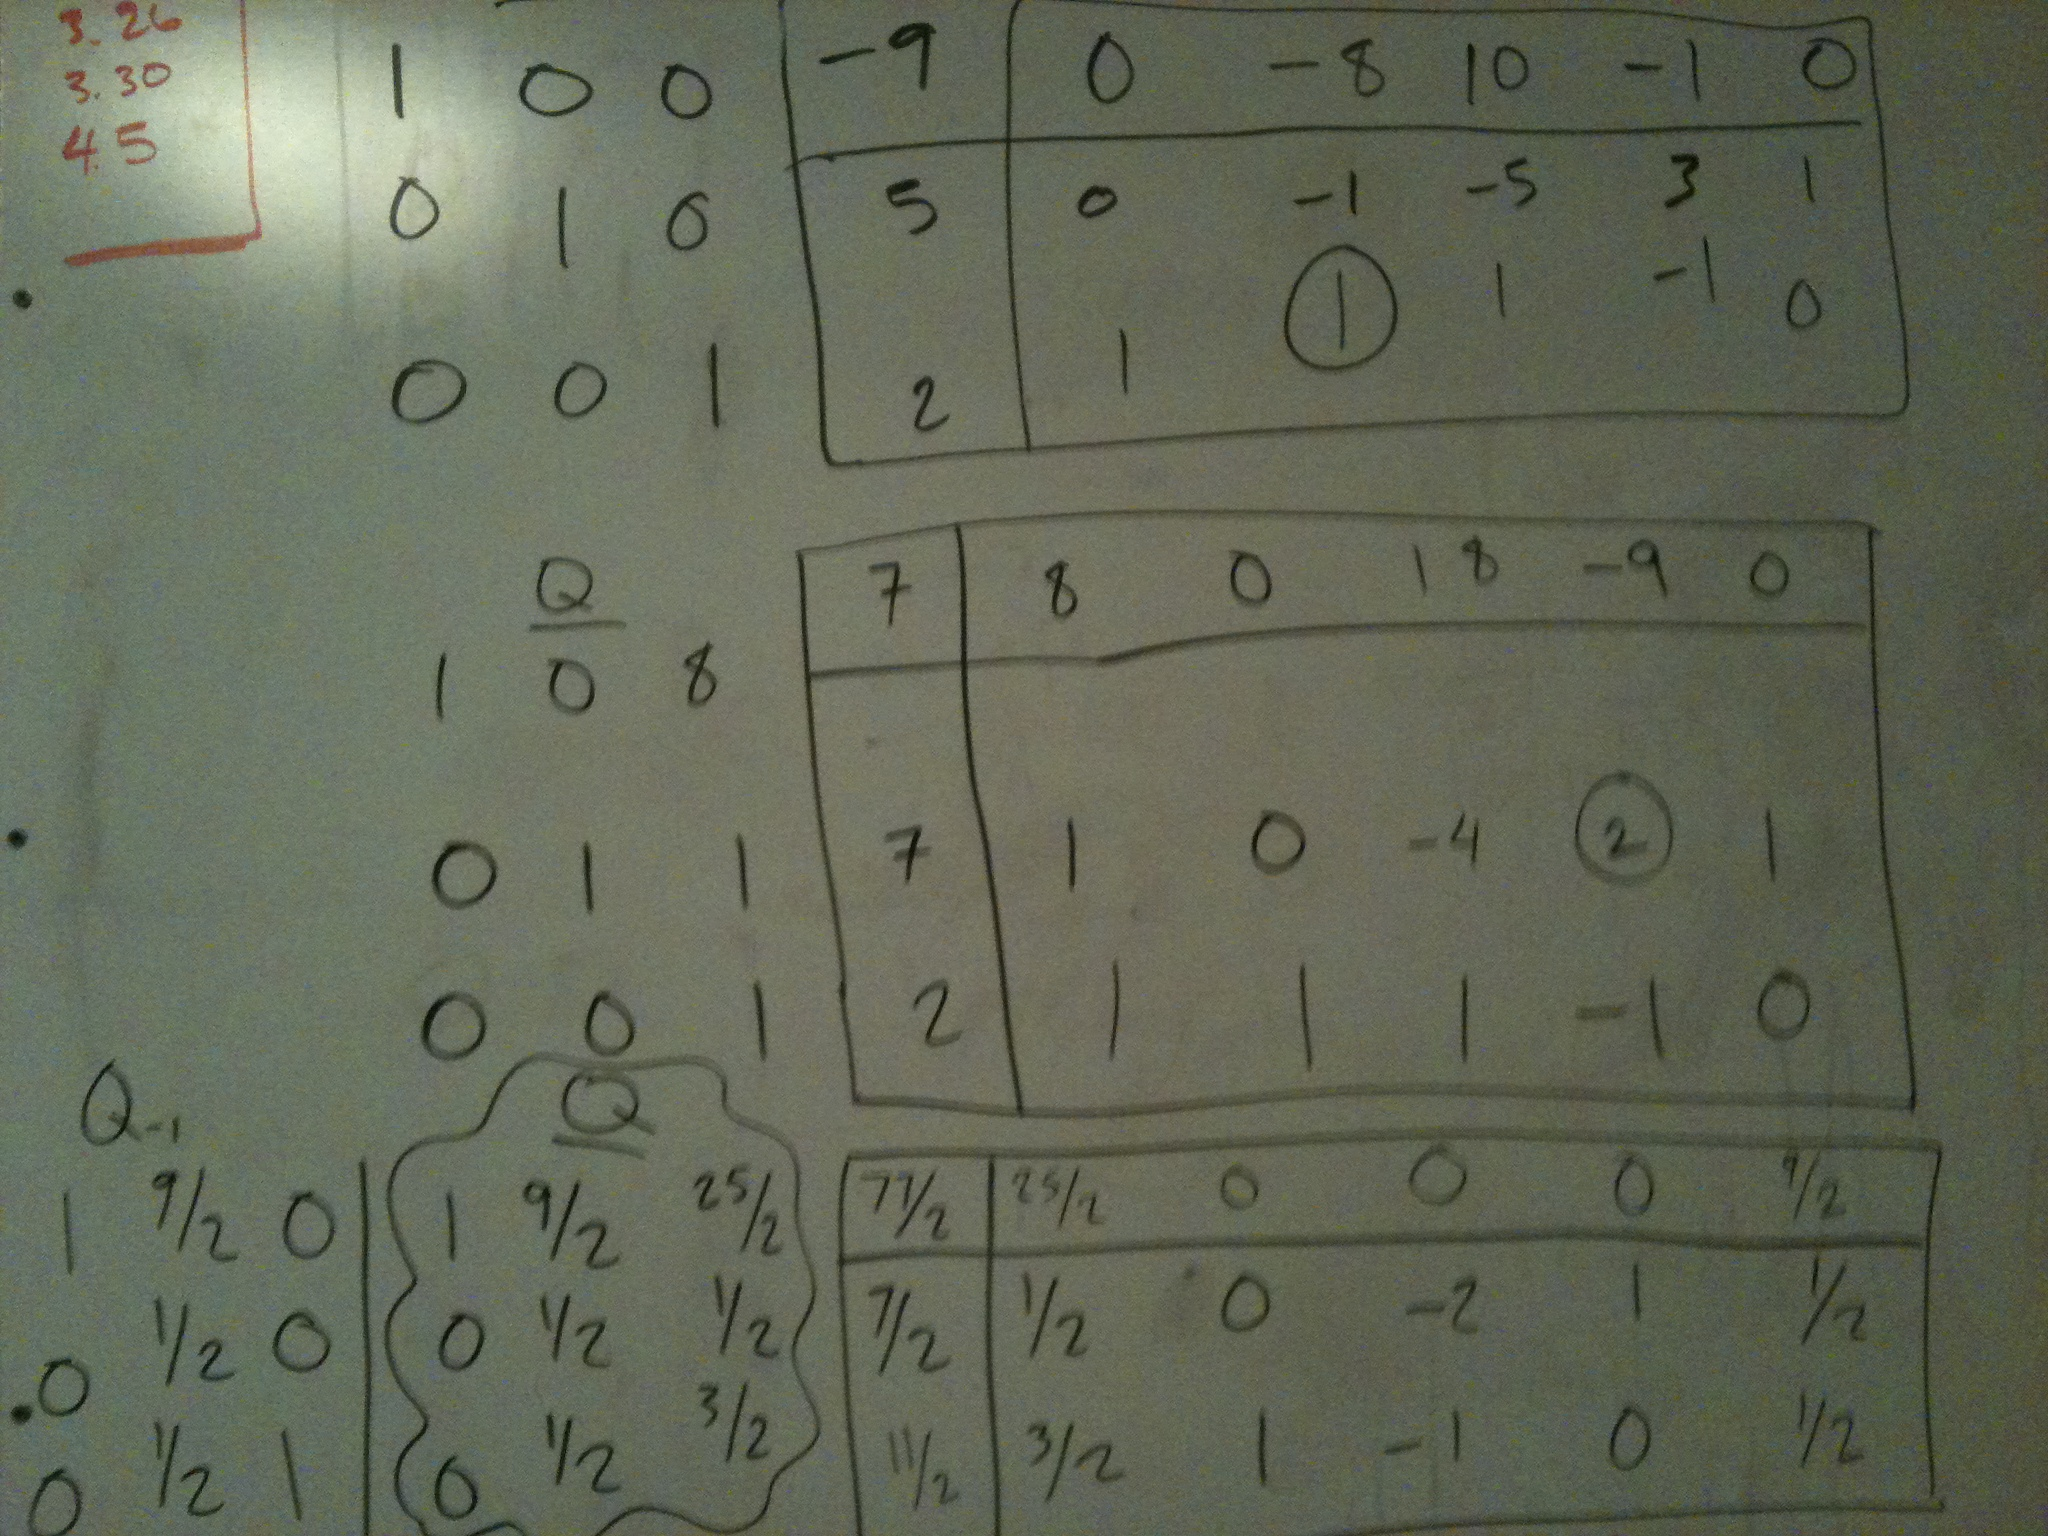
\includegraphics[width=14cm, height=14cm, keepaspectratio=true]{image/3_26.jpg}
\[
    Q = 
      \left[
        \begin{array}{c}
          1 \quad \dfrac{9}{2} \quad \dfrac{25}{2}\\\\ 
          0 \quad \dfrac{1}{2} \quad \dfrac{1}{2}\\\\
          0 \quad \dfrac{1}{2} \quad \dfrac{3}{2}\\
        \end{array}
      \right]
\]
\end{center}

\section*{3.30}
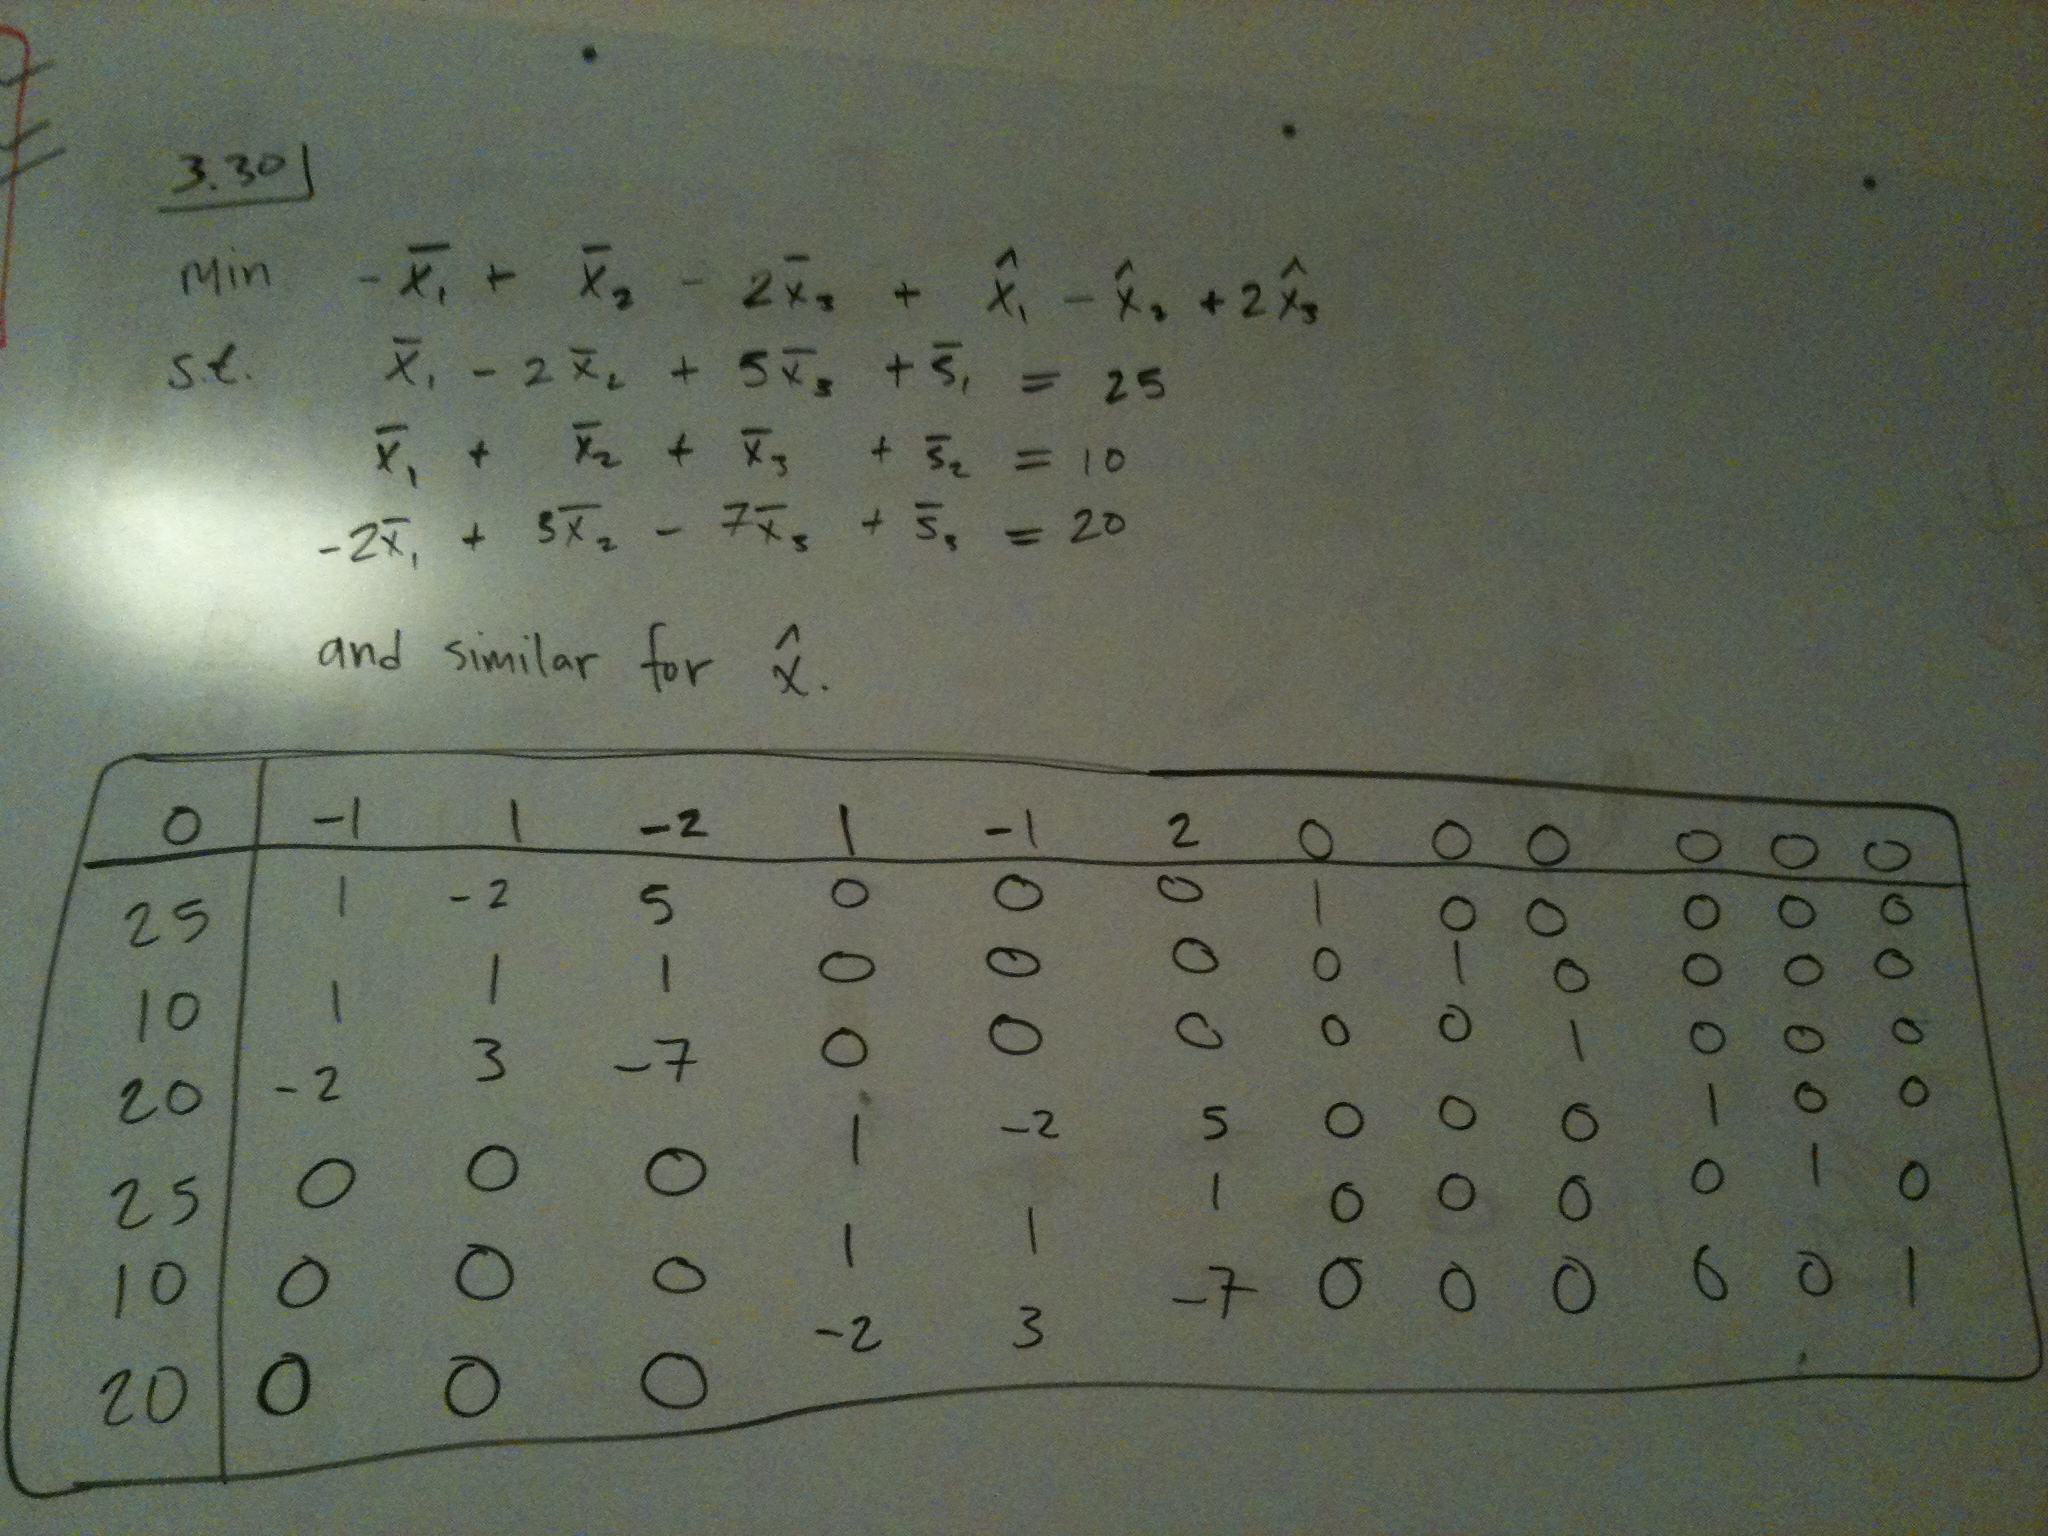
\includegraphics[width=14cm, height=14cm, keepaspectratio=true]{image/3_30.jpg}
Initial Tableau:
\begin{center}
\begin{tabular}{| c | c  c  c  c  c  c  c  c  c  c  c  c |}
\hline
0 & -1 & 1 & -2 & 1 & -1 & 2 & 0 & 0 & 0 & 0 & 0 & 0\\
\hline
25 & 1 & -2 & 5 & 0 & 0 & 0 & 1 & 0 & 0 & 0 & 0 & 0\\
10 & 1 & 1 & 1 & 0 & 0 & 0 & 0 & 1 & 0 & 0 & 0 & 0\\
20 & -2 & 3 & -7 & 0 & 0 & 0 & 0 & 0 & 1 & 0 & 0 & 0\\
25 & 0 & 0 & 0 & 1 & -2 & 5 & 0 & 0 & 0 & 1 & 0 & 0\\
10 & 0 & 0 & 0 & 1 & 1 & 1 & 0 & 0 & 0 & 0 & 1 & 0\\
20 & 0 & 0 & 0 & -2 & 3 & -7 & 0 & 0 & 0 & 0 & 0 & 1\\
\hline
\end{tabular}
\end{center}

Pivoting\dots
\begin{center}
\begin{tabular}{| c | c  c  c  c  c  c  c  c  c  c  c  c |}
\hline
10 & 0 & 2 & -1 & 1 & -1 & 2 & 0 & 1 & 0 & 0 & 0 & 0\\
\hline
15 & 0 & -3 & 4 & 0 & 0 & 0 & 1 & -1 & 0 & 0 & 0 & 0\\
10 & 1 & 1 & 1 & 0 & 0 & 0 & 0 & 1 & 0 & 0 & 0 & 0\\
40 & 0 & 5 & -5 & 0 & 0 & 0 & 0 & 2 & 1 & 0 & 0 & 0\\
25 & 0 & 0 & 0 & 1 & -2 & 5 & 0 & 0 & 0 & 1 & 0 & 0\\
10 & 0 & 0 & 0 & 1 & 1 & 1 & 0 & 0 & 0 & 0 & 1 & 0\\
20 & 0 & 0 & 0 & -2 & 3 & -7 & 0 & 0 & 0 & 0 & 0 & 1\\
\hline
\end{tabular}
\end{center}

Pivoting\dots
\begin{center}
\begin{tabular}{| c | c  c  c  c  c  c  c  c  c  c  c  c |}
\hline
13.75 & 0 & 1.25 & 0 & 1 & -1 & 2 & 0.25 & 0.75 & 0 & 0 & 0 & 0\\
\hline
3.75 & 0 & -0.75 & 1 & 0 & 0 & 0 & 0.25 & -0.25 & 0 & 0 & 0 & 0\\
6.25 & 1 & 1.75 & 0 & 0 & 0 & 0 & -0.25 & 1.25 & 0 & 0 & 0 & 0\\
58.75 & 0 & 1.25 & 0 & 0 & 0 & 0 & 1.25 & 0.75 & 1 & 0 & 0 & 0\\
25 & 0 & 0 & 0 & 1 & -2 & 5 & 0 & 0 & 0 & 1 & 0 & 0\\
10 & 0 & 0 & 0 & 1 & 1 & 1 & 0 & 0 & 0 & 0 & 1 & 0\\
20 & 0 & 0 & 0 & -2 & 3 & -7 & 0 & 0 & 0 & 0 & 0 & 1\\
\hline
\end{tabular}
\end{center}

Pivoting\dots
\begin{center}
\begin{tabular}{| c | c  c  c  c  c  c  c  c  c  c  c  c |}
\hline
20.4 & 0 & 1.25 & 0 & 0.333 & 0 & -0.333 & 0.25 & 0.75 & 0 & 0 & 0 & 0.333\\
\hline
3.75 & 0 & -0.75 & 1 & 0 & 0 & 0 & 0.25 & -0.25 & 0 & 0 & 0 & 0\\
6.25 & 1 & 1.75 & 0 & 0 & 0 & 0 & -0.25 & 1.25 & 0 & 0 & 0 & 0\\
58.8 & 0 & 1.25 & 0 & 0 & 0 & 0 & 1.25 & 0.75 & 1 & 0 & 0 & 0\\
38.3 & 0 & 0 & 0 & -0.333 & 0 & 0.333 & 0 & 0 & 0 & 1 & 0 & 0.667\\
3.33 & 0 & 0 & 0 & 1.67 & 0 & 3.33 & 0 & 0 & 0 & 0 & 1 & -0.333\\
6.67 & 0 & 0 & 0 & -0.667 & 1 & -2.33 & 0 & 0 & 0 & 0 & 0 & 0.333\\
\hline
\end{tabular}
\end{center}

And in optimal form:
\begin{center}
\begin{tabular}{| c | c  c  c  c  c  c  c  c  c  c  c  c |}
\hline
20.8 & 0 & 1.25 & 0 & 0.5 & 0 & 0 & 0.25 & 0.75 & 0 & 0 & 0.1 & 0.3\\
\hline
3.75 & 0 & -0.75 & 1 & 0 & 0 & 0 & 0.25 & -0.25 & 0 & 0 & 0 & 0\\
6.25 & 1 & 1.75 & 0 & 0 & 0 & 0 & -0.25 & 1.25 & 0 & 0 & 0 & 0\\
58.8 & 0 & 1.25 & 0 & 0 & 0 & 0 & 1.25 & 0.75 & 1 & 0 & 0 & 0\\
38 & 0 & 0 & 0 & -0.5 & 0 & 0 & 0 & 0 & 0 & 1 & -0.1 & 0.7\\
1 & 0 & 0 & 0 & 0.5 & 0 & 1 & 0 & 0 & 0 & 0 & 0.3 & -0.1\\
9 & 0 & 0 & 0 & 0.5 & 1 & 0 & 0 & 0 & 0 & 0 & 0.7 & 0.1\\
\hline
\end{tabular}
\end{center}

Has solution \(\bar{x} = (6.25, 0, 3.75)^T\) and \(\hat{x} = (0, 9, 1)^T \) 

\section*{4.5}
This answer is a series of two shots of my whiteboard. Answers a-h are labeled in the picture.\\
\begin{center}
  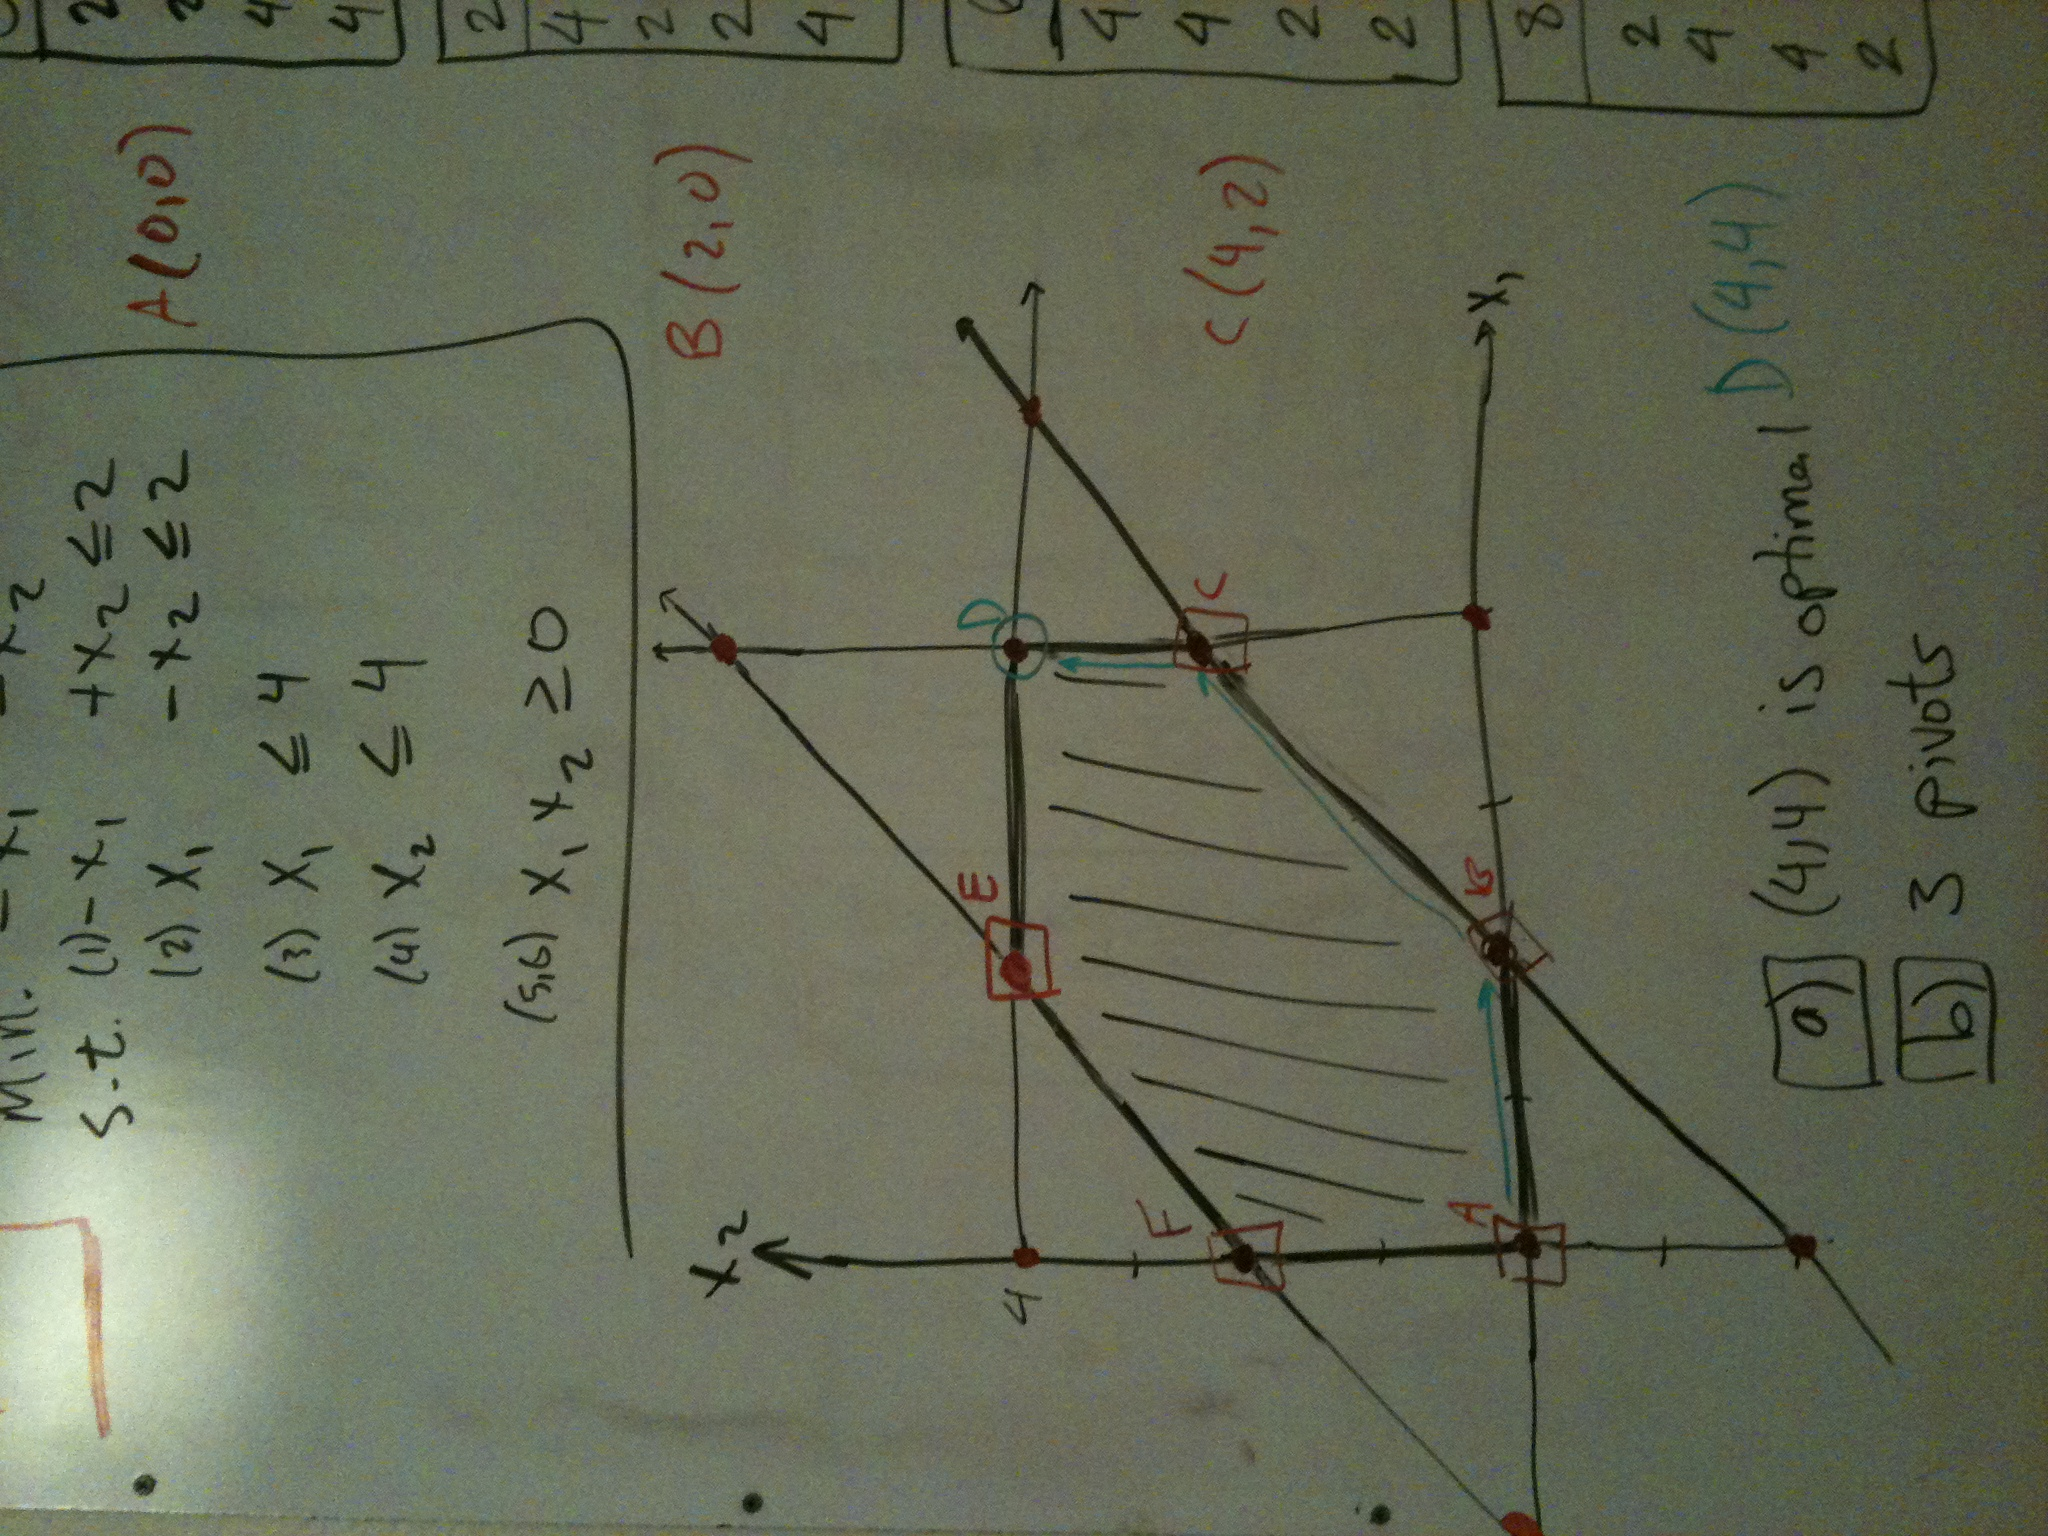
\includegraphics[width=14cm, height=14cm, keepaspectratio=true, angle=-90]{image/4_5_shot1.jpg}\\
  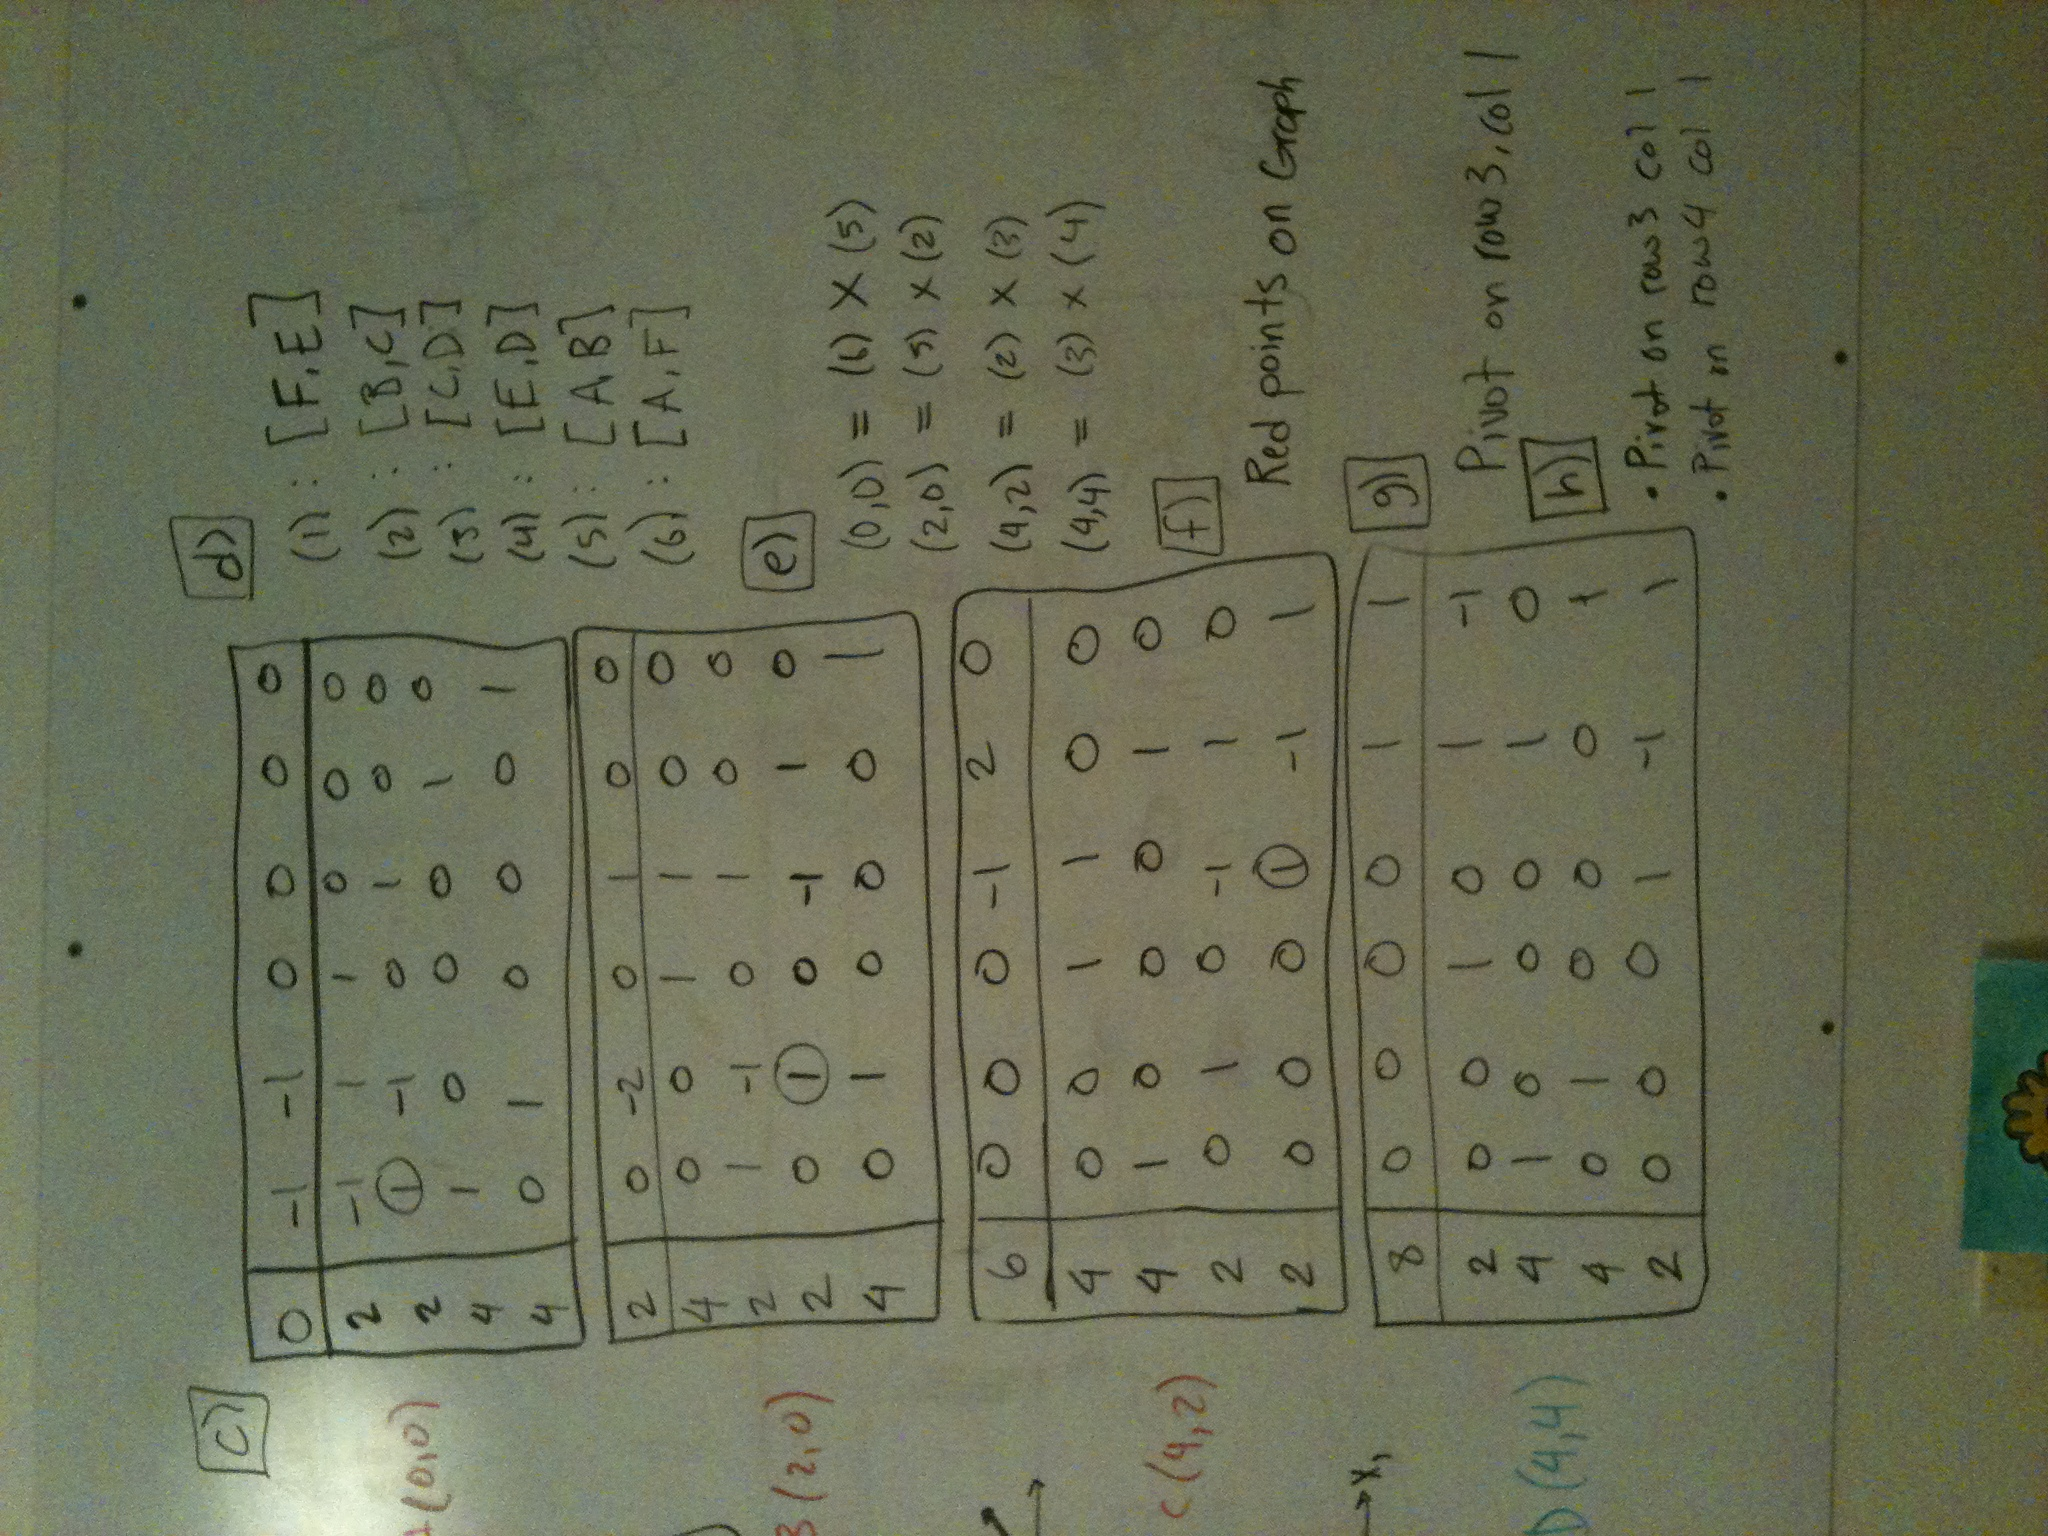
\includegraphics[width=14cm, height=14cm, keepaspectratio=true, angle=-90]{image/4_5_shot2.jpg}
\end{center}

\end{document}

